% !TeX root = ../main.tex

\addchap{Appendix} \label{chapter:appendix}

\refstepcounter{chapter} 
\section{Dataset Images}

\begin{figure}[h!tb]
\centering
\begin{subfigure}{1.0\textwidth}
  \centering
  \adjincludegraphics[width=1.0\linewidth,trim={0 0 0 0},clip]{figures/ds/ucf_train_full.png}
  \caption{Training set}
  \label{fig:ucf_train_full}
  \vspace{.1cm}
\end{subfigure}
\caption[UCF-101 Full Image Samples]{Randomly chosen and rescaled clip samples of size $160 \times 120$ from the UCF-101 dataset. There is only a very small portion of motion to see between one frame to the next, because the videos have a frame rate of \num{25} FPS.\\
\textit{(continues on next page)}}
\label{fig:ucf_full}
\end{figure}

\begin{figure}[h!tb]
\ContinuedFloat % continue from previous page
\centering
\begin{subfigure}{1.0\textwidth}
  \centering
  \adjincludegraphics[width=1.0\linewidth,trim={0 0 0 0},clip]{figures/ds/ucf_valid_full.png}
  \caption{Validation set}
  \label{fig:ucf_valid_full}
  \vspace{.1cm}
\end{subfigure}
\begin{subfigure}{1.0\textwidth}
  \centering
  \adjincludegraphics[width=1.0\linewidth,trim={0 0 0 0},clip]{figures/ds/ucf_test_full.png}
  \caption{Test set}
  \label{fig:ucf_test_full}
\end{subfigure}
\caption*{}
\end{figure}


\begin{figure}[h!tb]
\centering
\begin{subfigure}{1.0\textwidth}
  \centering
  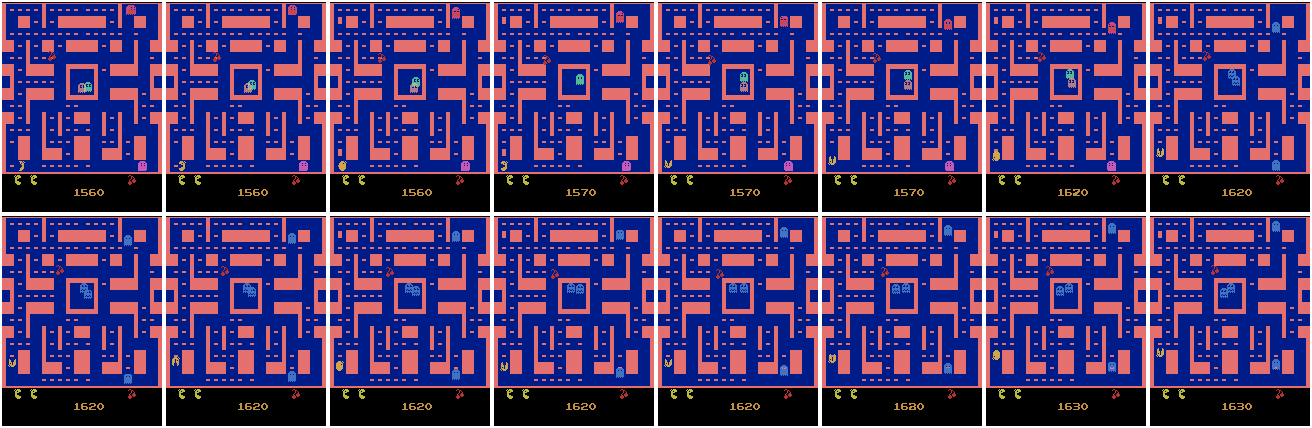
\includegraphics[width=1.0\linewidth]{figures/ds/pac_train_full.png}
  \caption{Training set}
  \label{fig:pac_train_full}
  \vspace{.1cm}
\end{subfigure}
\begin{subfigure}{1.0\textwidth}
  \centering
  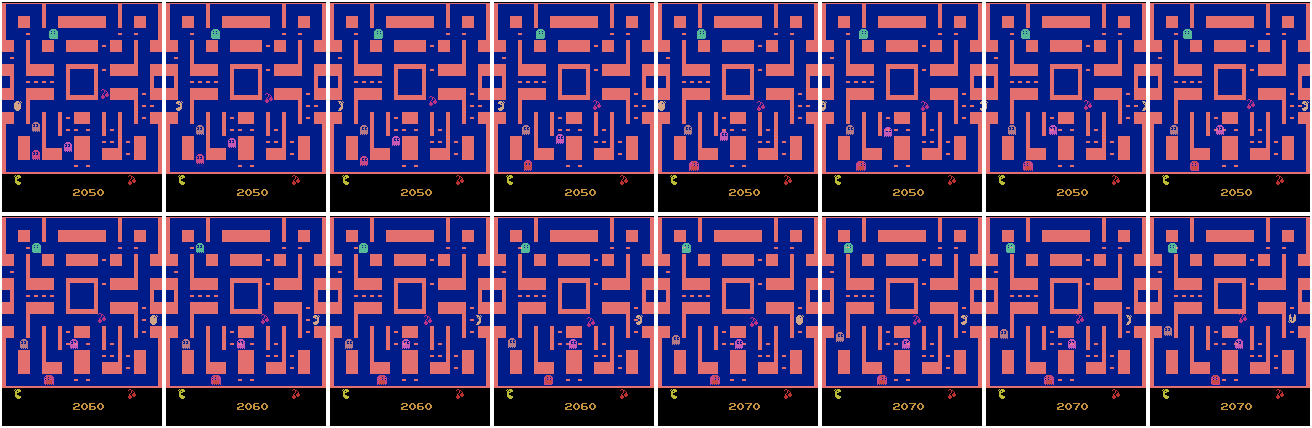
\includegraphics[width=1.0\linewidth]{figures/ds/pac_valid_full.png}
  \caption{Validation set}
  \label{fig:pac_valid_full}
  \vspace{.1cm}
\end{subfigure}
\begin{subfigure}{1.0\textwidth}
  \centering
  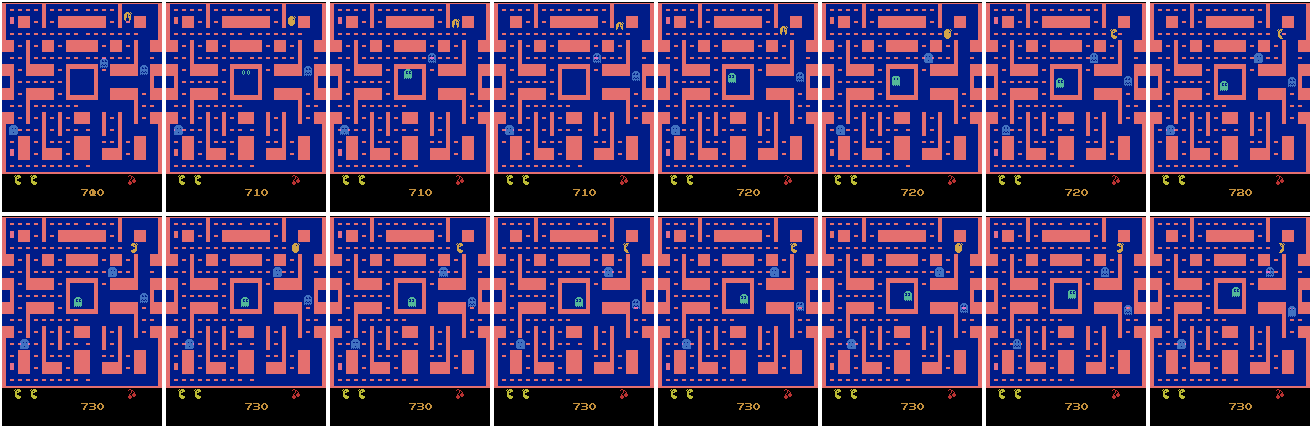
\includegraphics[width=1.0\linewidth]{figures/ds/pac_test_full.png}
  \caption{Test set}
  \label{fig:pac_test_full}
\end{subfigure}
\caption[MsPacman Full Image Samples]{Exemplary sequences of game recordings from MsPacman dataset that have been samples randomly from the different splits. Each shown clip has a length of \num{16} frames of size $160 \times 210$.}
\label{fig:pacman_full}
\end{figure}


\clearpage
\section{Further Frame Predictions}

\begin{figure}[htpb]
\centering
\begin{subfigure}{0.49\textwidth}
  \centering
  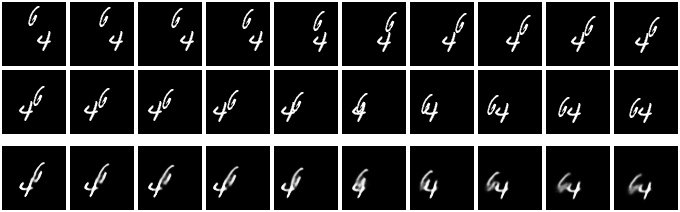
\includegraphics[width=0.92\linewidth]{figures/pred/mm/random/prediction-00.png}
  \caption{}
  \label{fig:mm-pred-random1}
  \vspace{.1cm}
\end{subfigure}%
\begin{subfigure}{0.49\textwidth}
  \centering
  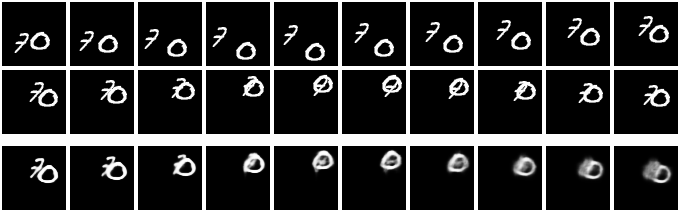
\includegraphics[width=0.92\linewidth]{figures/pred/mm/random/prediction-01.png}
  \caption{}
  \label{fig:mm-pred-random2}
  \vspace{.1cm}
\end{subfigure}
\begin{subfigure}{0.49\textwidth}
  \centering
  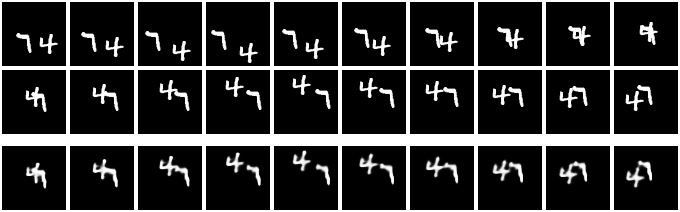
\includegraphics[width=0.92\linewidth]{figures/pred/mm/random/prediction-02.png}
  \caption{}
  \label{fig:mm-pred-random3}
\end{subfigure}
\begin{subfigure}{0.49\textwidth}
  \centering
  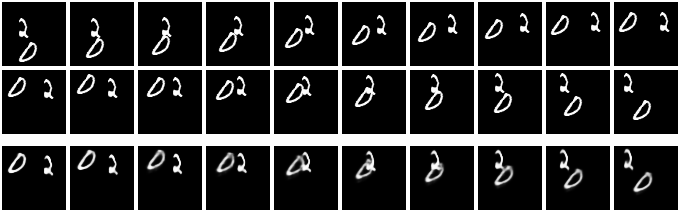
\includegraphics[width=0.92\linewidth]{figures/pred/mm/random/prediction-03.png}
  \caption{}
  \label{fig:mm-pred-random4}
\end{subfigure}
\caption[Random Prediction Samples on Moving MNIST]{Further random prediction samples on Moving MNIST. From top to bottom: ground truth input and output sequence; predicted sequence of our 2-layer model.} \label{fig:mm-pred-random}
\end{figure}

\begin{figure}[htpb]
\centering
\begin{subfigure}{0.5\textwidth}
  \centering
  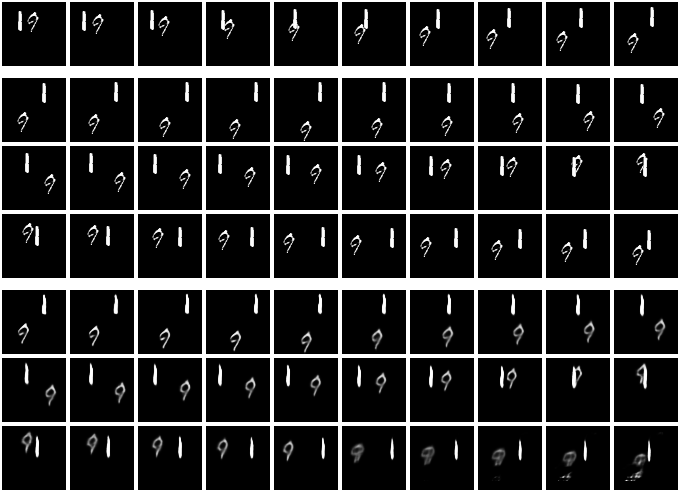
\includegraphics[width=0.9\linewidth]{figures/pred/mm/long/prediction-00.png}
  \caption{}
  \label{fig:mm-pred-long1}
\end{subfigure}%
\begin{subfigure}{0.5\textwidth}
  \centering
  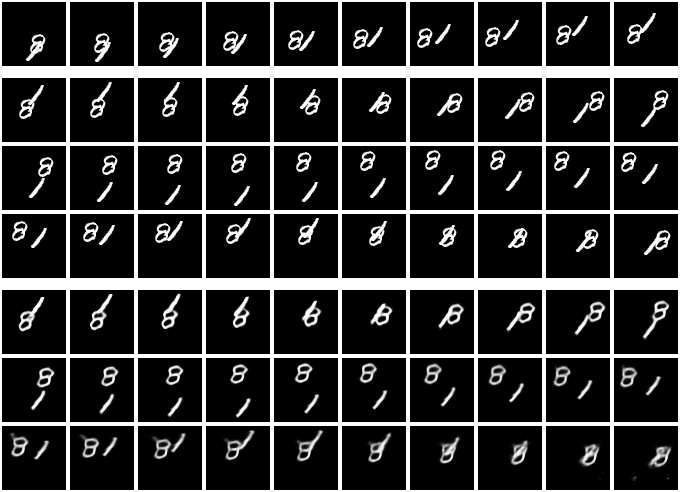
\includegraphics[width=0.9\linewidth]{figures/pred/mm/long/prediction-07.png}
  \caption{}
  \label{fig:mm-pred-long2}
\end{subfigure}
\caption[Long-Term Prediction on Moving MNIST]{Further out-of-domain runs on Moving MNIST. Our 2-layer model predicts 30 frames ahead, even that it is trained to predict 10 frames only. The spatio-temporal decoder is therefore unrolled for a longer time range.} \label{fig:mm-pred-long}
\end{figure}

\begin{figure}[h!tb]
\centering
\begin{subfigure}{0.49\textwidth}
  \centering
  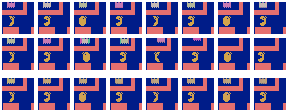
\includegraphics[width=0.92\linewidth]{figures/pred/pac/random/pred-01.png}
  \caption{}
  \label{fig:pac-pred-random_extra1}
\end{subfigure}%
\begin{subfigure}{0.49\textwidth}
  \centering
  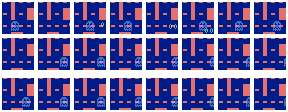
\includegraphics[width=0.92\linewidth]{figures/pred/pac/random/pred-02.png}
  \caption{}
  \label{fig:pac-pred-random_extra2}
\end{subfigure}
\caption[Prediction Samples on MsPacman]{Two further prediction examples of the 2-layer network on MsPacman. We have picked the best out of 8 random samples which contain at least some motion.} \label{fig:pac-pred-random_extra}
\end{figure}

\begin{figure}[htpb]
	\centering
	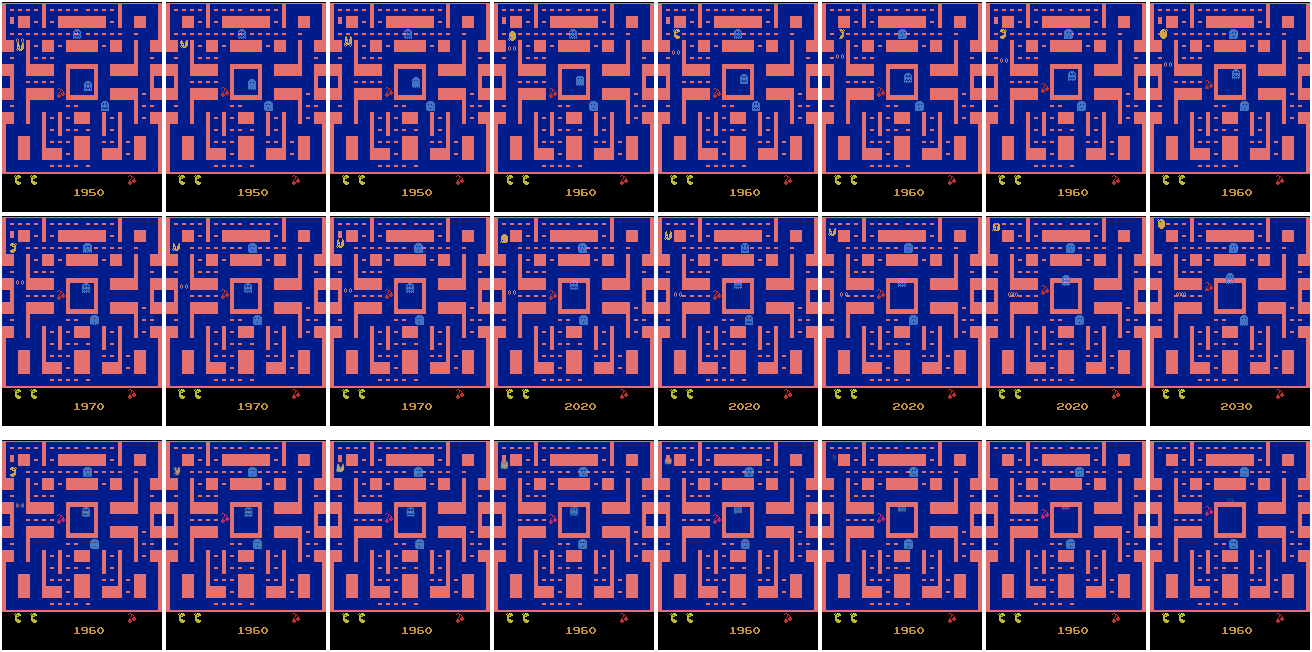
\includegraphics[width=1.0\linewidth]{figures/pred/pac/full/pred-01.png} 
	\caption[Full Screen Prediction on MsPacman]{Full screen prediction sample using our 2-layer model.} \label{fig:pac-pred-full2}
\end{figure}

\begin{figure}[htpb]
	\centering
	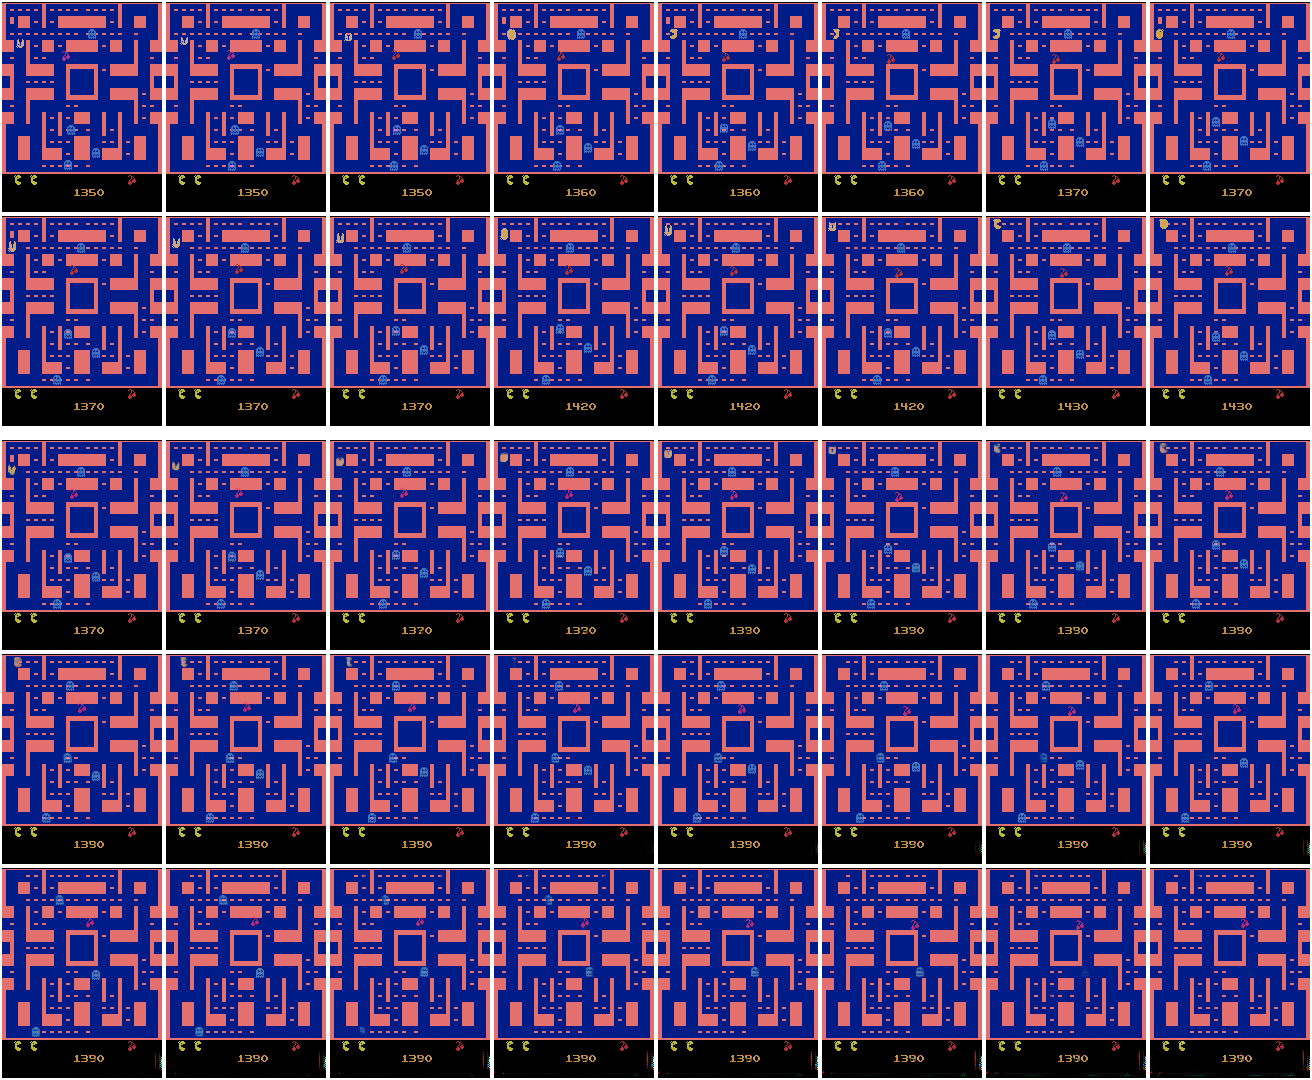
\includegraphics[width=1.0\linewidth]{figures/pred/pac/full-long/pred-00.png} 
	\caption[Long-Term Prediction on MsPacman]{Out-of-domain test using our 2-layer model to predict a longer-term future.} \label{fig:pac-pred-full-long}
\end{figure}



\begin{figure}[h!tb]
\centering
\begin{subfigure}{0.49\textwidth}
  \centering
  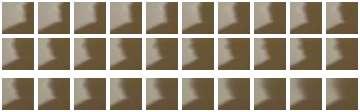
\includegraphics[width=0.92\linewidth]{figures/pred/ucf/random/pred-01.png}
  \caption{}
  \label{fig:ucf-random1a}
  \vspace{.1cm}
\end{subfigure}
\begin{subfigure}{0.49\textwidth}
  \centering
  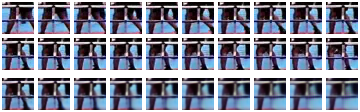
\includegraphics[width=0.92\linewidth]{figures/pred/ucf/random/pred-02.png}
  \caption{}
  \label{fig:ucf-random1b}
  \vspace{.1cm}
\end{subfigure}
\begin{subfigure}{0.49\textwidth}
  \centering
  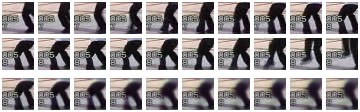
\includegraphics[width=0.92\linewidth]{figures/pred/ucf/random/pred-03.png}
  \caption{}
  \label{fig:ucf-random1c}
  \vspace{.1cm}
\end{subfigure}
\begin{subfigure}{0.49\textwidth}
  \centering
  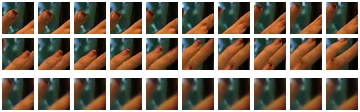
\includegraphics[width=0.92\linewidth]{figures/pred/ucf/random/pred-05.png}
  \caption{}
  \label{fig:ucf-random1d}
  \vspace{.1cm}
\end{subfigure}
\caption[TBD]{tbd.}
\label{fig:ucf-random1}
\end{figure}


\begin{figure}[htpb]
	\centering
	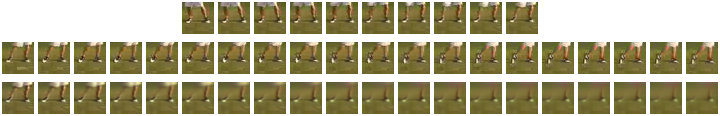
\includegraphics[width=1.0\linewidth]{figures/pred/ucf/long/pred-00.png} 
	\caption[TBD]{tbd.} \label{fig:ucf-long2}
\end{figure}


\begin{figure}[h!tb]
\centering
\begin{subfigure}{1.0\textwidth}
  \centering
  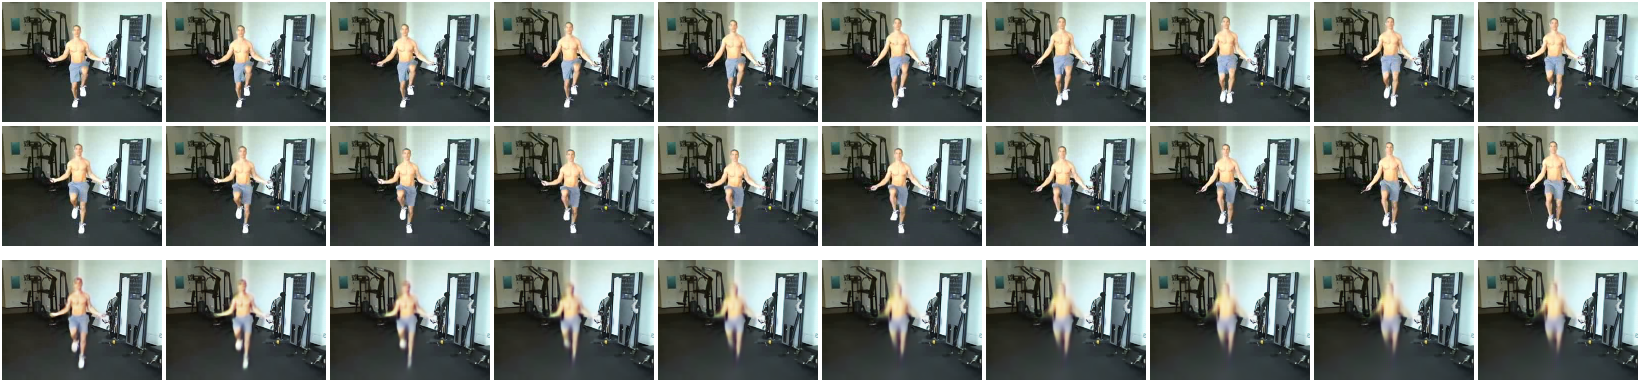
\includegraphics[width=1.0\linewidth]{figures/pred/ucf/full/pred-02.png}
  \caption{}
  \label{fig:ucf-full2a}
  \vspace{.1cm}
\end{subfigure}
\begin{subfigure}{1.0\textwidth}
  \centering
  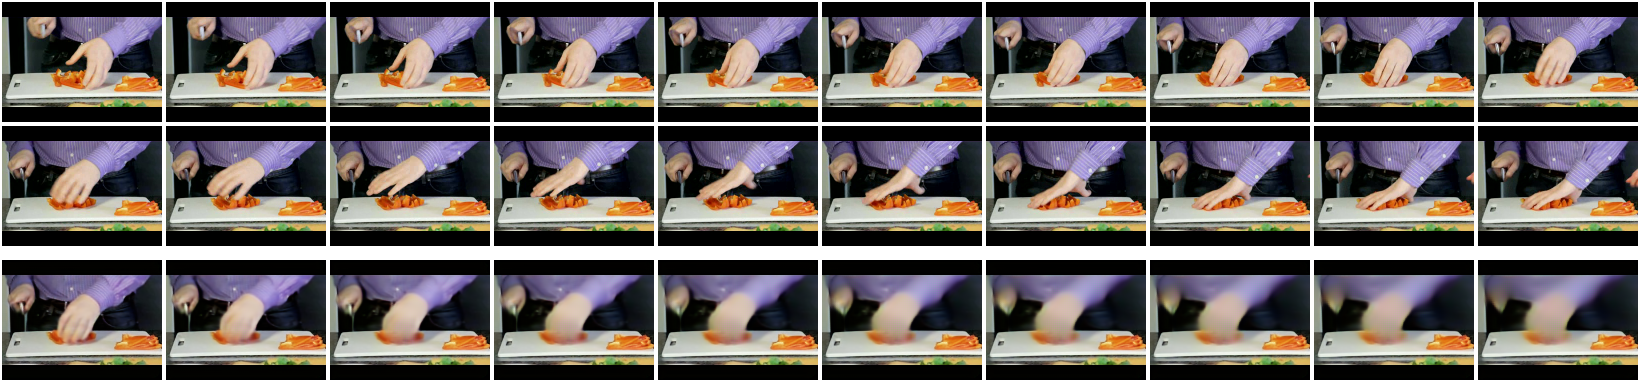
\includegraphics[width=1.0\linewidth]{figures/pred/ucf/full/pred-03.png}
  \caption{}
  \label{fig:ucf-full2b}
  \vspace{.1cm}
\end{subfigure}
\caption[TBD]{tbd.}
\label{fig:ucf-full2}
\end{figure}



\clearpage
\section{Code Listings}

\begin{figure}[h!tb]
  \lstinputlisting[language=PythonEx]{code/model.py}
  \caption[Code: Convolutional Autoencoder]{Example implementation of a convolutional autoencoder model.}\label{code:model}
\end{figure}

